%%%%%%%%%%%%%%%%%%%%%%%%%%%%%%%%%%%%%%%%%
% Programming/Coding Assignment
% LaTeX Template
%
% This template has been downloaded from:
% http://www.latextemplates.com
%
% Original author:
% Ted Pavlic (http://www.tedpavlic.com)
%
% Note: 
% The \lipsum[#] commands throughout this template generate dummy text
% to fill the template out. These commands should all be removed when 
% writing assignment content.
%
% This template uses a Perl script as an example snippet of code, most other
% languages are also usable. Configure them in the "CODE INCLUSION 
% CONFIGURATION" section.
%
%%%%%%%%%%%%%%%%%%%%%%%%%%%%%%%%%%%%%%%%%
 
%----------------------------------------------------------------------------------------
%	PACKAGES AND OTHER DOCUMENT CONFIGURATIONS
%----------------------------------------------------------------------------------------

\documentclass[table,11pt]{article}

\usepackage{fancyhdr} % Required for custom headers
\usepackage{lastpage} % Required to determine the last page for the footer
\usepackage{extramarks} % Required for headers and footers
\usepackage[usenames,dvipsnames]{xcolor} % Required for custom colors
\usepackage{graphicx} % Required to insert images
\usepackage{listings} % Required for insertion of code
\usepackage{courier} % Required for the courier font
\usepackage{url}
\usepackage{paralist}
\usepackage{pgfgantt}

\usepackage{booktabs}
\usepackage{multirow}
\usepackage{array}
\usepackage{arydshln}

\usepackage[pdfpagemode={UseOutlines},bookmarks=true,bookmarksopen=true,
   bookmarksopenlevel=0,bookmarksnumbered=true,hypertexnames=false,
   colorlinks,linkcolor={blue},citecolor={blue},urlcolor={red},
   pdfstartview={FitV},unicode,breaklinks=true]{hyperref}
    
    
\usepackage{todonotes}
\newcommand{\todojc}[1]{\todo[inline]{JC: #1}}
   
% Margins
\topmargin=-0.45in
\evensidemargin=0in
\oddsidemargin=0in
\textwidth=6.5in
\textheight=9.0in
\headsep=0.25in

\linespread{1.1} % Line spacing

% Set up the header and footer
\pagestyle{fancy}
\lhead{\hmwkAuthorNameShort} % Top left header
\chead{\hmwkTitle} % Top center head
\rhead{} % Top right header
\lfoot{} % Bottom left footer
\cfoot{} % Bottom center footer
\rfoot{Page\ \thepage\ of\ \protect\pageref{LastPage}} % Bottom right footer
\renewcommand\headrulewidth{0.4pt} % Size of the header rule
\renewcommand\footrulewidth{0.4pt} % Size of the footer rule

%\setlength\parindent{0pt} % Removes all indentation from paragraphs

%----------------------------------------------------------------------------------------
%	CODE INCLUSION CONFIGURATION
%----------------------------------------------------------------------------------------
\definecolor{mygreen}{rgb}{0,0.6,0}
\definecolor{mygray}{rgb}{0.5,0.5,0.5}
\definecolor{mymauve}{rgb}{0.58,0,0.82}
\definecolor{mylisting}{rgb}{1,0.98,0.756}

\lstset{ %
  backgroundcolor=\color{mylisting},   % choose the background color; you must add \usepackage{color} or \usepackage{xcolor}
  basicstyle=\footnotesize,        % the size of the fonts that are used for the code
  breakatwhitespace=false,         % sets if automatic breaks should only happen at whitespace
  breaklines=true,                 % sets automatic line breaking
  captionpos=t,                    % sets the caption-position to bottom
  commentstyle=\color{mygreen},    % comment style
  deletekeywords={...},            % if you want to delete keywords from the given language
  escapeinside={\%*}{*)},          % if you want to add LaTeX within your code
  extendedchars=true,              % lets you use non-ASCII characters; for 8-bits encodings only, does not work with UTF-8
  frame=single,                    % adds a frame around the code
  keepspaces=true,                 % keeps spaces in text, useful for keeping indentation of code (possibly needs columns=flexible)
  keywordstyle=\color{blue},       % keyword style
  language=bash,                 % the language of the code
  morekeywords={*,...},            % if you want to add more keywords to the set
  numbers=left,                    % where to put the line-numbers; possible values are (none, left, right)
  numbersep=5pt,                   % how far the line-numbers are from the code
  numberstyle=\tiny\color{mygray}, % the style that is used for the line-numbers
  rulecolor=\color{black},         % if not set, the frame-color may be changed on line-breaks within not-black text (e.g. comments (green here))
  showspaces=false,                % show spaces everywhere adding particular underscores; it overrides 'showstringspaces'
  showstringspaces=false,          % underline spaces within strings only
  showtabs=false,                  % show tabs within strings adding particular underscores
  stepnumber=2,                    % the step between two line-numbers. If it's 1, each line will be numbered
  stringstyle=\color{mymauve},     % string literal style
  tabsize=2,                       % sets default tabsize to 2 spaces
  title=\lstname                   % show the filename of files included with \lstinputlisting; also try caption instead of title
}




\renewcommand{\arraystretch}{1.5}
\newcolumntype{C}[0]{>{\centering\arraybackslash}m{0.75cm}}
\newcommand{\critical}[2]{\multicolumn{#1}{|c|}{\cellcolor{red!65}#2}}


\newcommand{\includecode}[2]{\lstinputlisting[caption=#2,captionpos=t,language=C]{code/#1}}


%----------------------------------------------------------------------------------------
%	NAME AND CLASS SECTION
%----------------------------------------------------------------------------------------

\newcommand{\hmwkTitle}{Nios Code Generation Specification} % Assignment title
\newcommand{\hmwkDueDate}{\today} % Due date
\newcommand{\hmwkClass}{} % Course/class
\newcommand{\hmwkClassTime}{} % Class/lecture time
\newcommand{\hmwkClassInstructor}{} % Teacher/lecturer
\newcommand{\hmwkAuthorName}{Jonah Caplan} % Your name
\newcommand{\hmwkAuthorNameShort}{Caplan} % Your name

%----------------------------------------------------------------------------------------
%	TITLE PAGE
%----------------------------------------------------------------------------------------

\title{
\vspace{2in}
\textmd{\textbf{\hmwkTitle}}\\
\vspace{3in}
}

\author{\textbf{\hmwkAuthorName}}
\date{} % Insert date here if you want it to appear below your name



%----------------------------------------------------------------------------------------

\begin{document}

\maketitle
\thispagestyle{empty}
\newpage
\setcounter{page}{1}

%------------------------------------------------------------------------------------
\section{Introduction}

The aim of this project is to develop an infrastructure for the automatic generation of C code for multicore Nios systems. We assume that an external model based design approach is used to generate control algorithms and that C code for these computations have already been generated in separate files (e.g. Simulink). The purpose of this tool is to efficiently map the control system onto an arbitrary platform while taking into account non-functional requirements such as deadlines, data flow, and criticality. The user must only specify the requirements for the system at a high level of abstraction and all intermdeiate code will be automatically generated. 

This tool will not initially be geared towards solving codesign problems. We will assume a static hardware platform and ocnsider changing software requirements only. In order to facilitate later expansions, the tool will require the specification of the hardware in terms of generic model parameters. The task-mapping procedure will be platform independent and solve the problem generically even if we do not currently take advantage of this feature.

This document will provide the specification for the currently supported hardware models, the platform built from these components currently under study, the application models for analysis of software requirements, the mapping procedure combining both hardware and software models to generate a schedule, and the abstract template requirements for code generation.



%%%%%%%%%%%%%%%%%%%%%%%%%%%%%%%%%%%%%%%%%%%%%%%%%%%%%%%%%%%%%%%%%%%%%%%%%%%%%%%%%%%%%%%%%%%%%%%%%%%%%%%%%%%%%%%%
\section{Tool Structure}

This key to success for this project in the given time frame is to leverage open source, take advantage of the wealth of prior work in the field from the 1990s in synchronous language design, and more current work on automated DSE and code generation. Furthermore, the wealth of generated code that describes the platform, as well as a very well structured RTOS uC/OS-II integrated into the BSP make the job of template development and hardware platform specification much easier. While the code can be a bit cumbersome to navigate for a human user because it is generated, this actually makes it much easier to parse for an automated process.


Figure \ref{f:tool_arch} depicts the tool architecture. 
From this figure we can begin to derive a timeline for development by identifying and prioritizing milestones. 
% Figure \ref{f:gantt} depicts an equivalent Gantt chart.

\begin{enumerate}
\item Define model classes for application and processors.
\item Integrate models with GA library to build task mapper.
\item Test mapper extensively with randomly generated task graphs, including timing data and fault-tolerance requirements.
\item Write RTOS templates.
  \begin{enumerate}
  \item Deconstruct existing code into discrete units with well-defined functionality.
  \item Formalize inter-core communication protocols.
  \item Write new templates for non-existing features (e.g. killing erroneous tasks, setting MPU parameters).
  \item Rewrite all drivers for fingerprint unit, comparator and TLB.
  \end{enumerate}
\item Build code generation tool.
\item Write WCET estimation tool.
\item Define QSYS naming conventions and write system.h BSP parser.
\item Write language specification for high level model input.
\item Write scanner/parser using SableCC3 to build abstract Java application model from user input. 
\end{enumerate}




% \newpage


\begin{figure}[h]
\centering
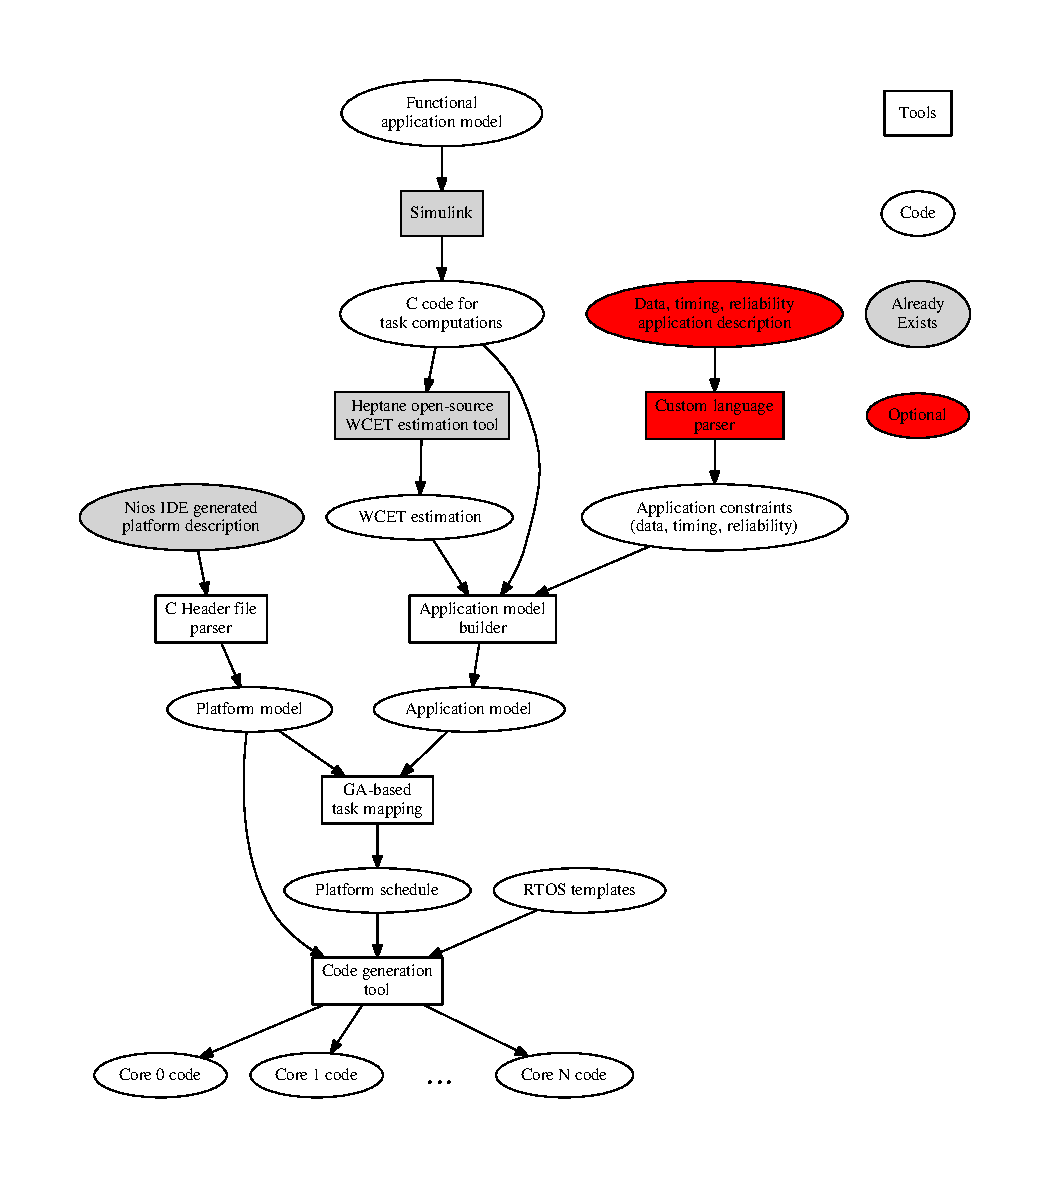
\includegraphics[scale=0.8]{figures/tool_arch}
\caption{The proposed tool architecture.}
\label{f:tool_arch}
\end{figure}
% 
% 
% \begin{figure}[h]
% % \begin{center}
% \begin{ganttchart}{1}{8}
% % \gantttitle{Development Timeline}{8} \\
% \gantttitlelist{1,...,8}{1} \\
% \ganttbar{Define Model Classes}{1}{1} \\
% \ganttlinkedbar{Build task mapper}{2}{2} \\
% \ganttlinkedbar{Write RTOS templates}{3}{3} \\
% \ganttlinkedbar{Code generation tool}{4}{4} \\
% \ganttlinkedbar{Port Heptane}{5}{5} \\
% \ganttlinkedbar{Nios BSP parser}{6}{6} \\
% \ganttlinkedbar{Specify application modelling language}{7}{7} \\
% \ganttlinkedbar{Scanner/Parser for modelling language}{8}{8} \\
% % \ganttgroup{Group 1}{1}{7} \\
% % \ganttlinkedbar{Task 2}{3}{7} \ganttnewline
% % \ganttbar{Final Task}{8}{12}
% 
% \end{ganttchart}
% % \end{center}
% \caption{Timeline for development of main tool components}
% \label{f:gantt}
% \end{figure}

%%%%%%%%%%%%%%%%%%%%%%%%%%%%%%%%%%%%%%%%%%%%%%%%%%%%%%%%%%%%%%%%%%%%%%%%%%%%%%%%%%%%%%%%%%%%%%%%%%%%%%%%%%%%%%%%
\section{Hardware Model}
Hardware models are specified using an object-oriented semantics. The system is divided into hierarchical levels that are interpreted using static scoping rules to aid in the specification of larger models. 

The cost in tiucme of transmitting over communication channel models is omitted at this stage beyond specifying the connections between elements. Issues related to resource arbitration and interference are also not considered. The underlying infrastructure is assumed to be sufficiently quick and deterministic.

There are four categories of hardware models in the system: processor cores, peripheral cores, and memory and buses.

\subsection{Processor cores}
All processor cores are assumed to operate at the same clock frequency. Their parameters are determined during hardware design and are not altered during software mapping. They can be extracted from the \emph{system.h} file generated from the {.sopcinfo} file by the Nios IDE during BSP generation.

Processor parameters are:
\begin{enumerate}
\item \emph{Fault-tolerant}: While we do not have access to safety-critical Nios licenses, they do exist. We assume that a core can be designated as fault tolerant (FT) and that a cost is associated with fault tolerance (due to licensing, size, resource utilization, power consumption as appropriate for the scenario) and that it is therefore necessary to have fewer FT cores in the system.

\item \emph{Scratchpad}: 
The processor must have a scratchpad in order to use fingerprinting as an error detection mechanism under our current implementation. The relevant parameters for the scratchpad will be listed separately.

\item \emph{Timer}: 
The system timer will dictate the minimum period for events in the system. The timer period is statically assigned when specifying the hardware design in QSYS.

\item \emph{Fingerprint Unit}: 
Fingerprint units will be necessary to allow the monitoring of processing cores (PC), i.e. those cores lacking FT capabilities, by a FT core.
 
\item \emph{Data and instruction cache}: 
It may be necessary to disable data and/or instruction caches while executing critical tasks. It must be known if the processor is equipped with either.

\item \emph{DMA}:
A single channel DMA will be used to shuttle critical data in and out of the scratchpads.

\item \emph{MPU}:
An MPU will be required to ensure that each core is unable to maintain partitions between each core.

\item \emph{Shared memory}:
Shared memory space will be required to load instructions

\item \emph{Interrupt signals}:
The processor model must specify the actively connected interrupt signals.

\end{enumerate}

This is a very general model of the processor. The mapping of tasks to cores will take place considering a very high level model of the system. The lower level parameters will only be used for code generation purposes. For the processor model, it is sufficient to consider whether or not each of these components are available. The details of each component will be hidden from the mapping problem at this higher level of abstraction.

\subsection{Memory}
Local scratchpads will be required for each core as well as shared main memory. A memory is defined simply as a start and end address. Memory latencies are not modelled. A memory model will also keep track of what other modules are connected to it.

There will be two partitioned sections of shared main memory. One to access common functions for redundant task executions and another for message passing between cores.

\subsection{Peripherals}
Certain details about the peripherals such as control registers will be entirely encapsulated in the template objects for the code generation phase. The higher level concerns that will dictate how these registers are sit will be included in the object representation of each peripheral. Mappings from the higher level concerns to code generation rules will be specified.

\subsubsection{Timer}
The frequency of the system level timer must be known in order to define the minimum resolution of time in the application model. Preexisting drivers exist and macros are generated by the Nios IDE to manage the timer. All relevant macros can be extracted from the generated code.

\subsubsection{Fingerprint Unit} 
The fingerprint unit has the following features: maximum stack depth, statically set during hardware design, and block length size. The setting of

\subsubsection{Memory Protection Unit}

\subsubsection{Comparator}

\subsubsection{DMA}

\subsubsection{$\mu$TLB}
 

%%%%%%%%%%%%%%%%%%%%%%%%%%%%%%%%%%%%%%%%%%%%%%%%%%%%%%%%%%%%%%%%%%%%%%%%%%%%%%%%%%%%%%%%%%%%%%%%%%%%%%%%%%%%%%%%

\section{Application Model}

\subsection{Functional decomposition}
An extension to MPSoCs is proposed to the application model and response-time analysis presented by Baruah, Burns and Davis in \cite{baruah2011response}. Tasks are defined in the uniprocessor case by the tuple $\tau_i= <T_i,D_i,\overrightarrow{C_i},L_i>$. Tasks are assumed to be independent and periodic. It may be beneficial in a multicore system to consider core allocation at a finer granularity. Tasks may be composed of several functions with dataflow dependencies between them. It may be desirable to allocate several cores to a single task in order to allow the parallel execution of these functions. We will only consider a two core case as an example to simplify the discussion.

The problem of deciding whether or not to execute a task on a specific core, or on both cores, and how to assign functions within a task to a given core will probably need to be explored using standard DSE techniques such as a genetic algorithm as the size of the space will grow very quickly (\emph{how quickly?}). \textbf{The question is whether or not allowing the division of a task into subcomponents and to allow the acquisition of more than one resource at a time by a single task allows more systems with higher utilization to pass schedulability tests than standard techniques.}

Consider the complex task graph in Figure \ref{f:complex_tg}. Each function has some WCET associated with it. Suppose the WCET of the task is 110ms and is decomposed as in Table \ref{t:complex_tg}. It is possible to execute this task on two resources with the mapping shown in Figure \ref{f:distr_tg}. A difference of 30ms is achieved. Communication overhead could be modeled by including a bus as a processing element and to insert tasks into the graph to model the communication overhead. For now the inter-core communication overhead is assumed to be negligible.  
 

\begin{figure}[h]
\centering
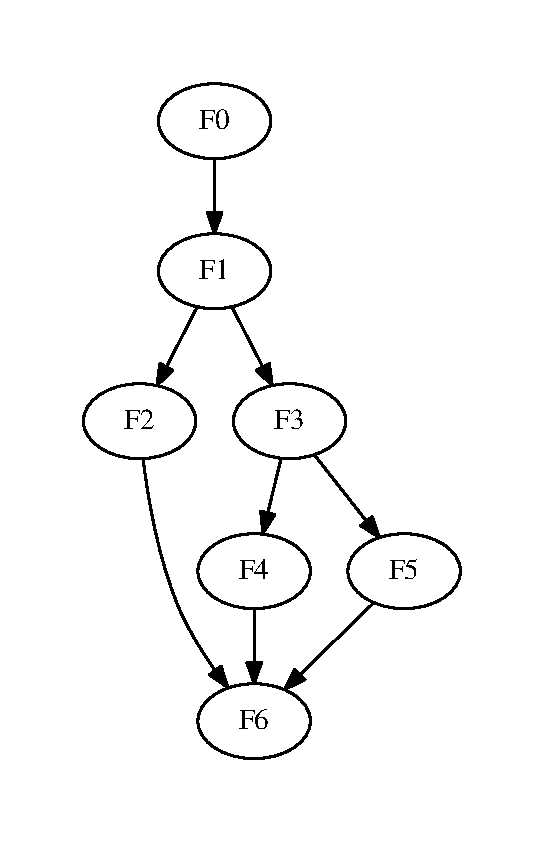
\includegraphics[scale=0.5]{figures/complex_tg.pdf}
\caption{Example of task decomposition into functions with dataflow precedence relations.}
\label{f:complex_tg}
\end{figure}

\begin{table}
\centering
\begin{tabular}{l | r}
Function & WCET \\
\hline
F0 & 20 \\
F1 & 10 \\
F2 & 10 \\
F3 & 10 \\
F4 & 20 \\
F5 & 30 \\ 
F6 & 10 \\
\hline
Total & 110
\end{tabular}
\caption{WCET derivation for the task in Figure \ref{f:complex_tg}}
\label{t:complex_tg}
\end{table}

\begin{figure}
\begin{tabular}{l|*{11}{C:}}
Time & 10 & 20 & 30 & 40 & 50 & 60 & 70 & 80 & 90 & 100 & 110\\
\hline 
& & & & & & & & & & & \\
\cline{2-7} \cline{9-9}
CPU1 & \multicolumn{2}{c|}{F0} &\multicolumn{1}{c|}{F1}  & \multicolumn{1}{|c|}{F2} & \multicolumn{2}{|c|}{F4} & &\multicolumn{1}{|c|}{F6} & & &\\
\cline{2-7} \cline{9-9}
& & & & & & & & & & &\\
\cline{5-8} 
%When the task edges are touching can leave out one of the '|' characters in
CPU2 & & & & \multicolumn{1}{|c|}{F3} & \multicolumn{3}{|c|}{F5}& & &&\\
\cline{5-8} 
\hline
\end{tabular}
\caption{Possible mapping for distributed task onto two cores.}
\label{f:distr_tg}
\end{figure}

Now consider a set of tasks $\tau_i \in T$ each of which can be optionally decomposed and distributed in such a fashion. The decision of which tasks to decompose will best be left to a DSE approach. The analysis that follows assumes that a strategy has already been chosen. The following discussion will apply SMC as a first step to demonstrate how the RTA can be accomplished using standard analysis. The mapping in Figure \ref{f:distr_tg} is reexpressed as a transformed CFG in Figure \ref{f:trans_cfg}. The communication overhead is now explicitly modeled (but can be given an execution time C=0). The program is divided into serial and parallel chunks. For example $S_0=\{F_0,F_1\}$ and the first parallel branch $P_{0.0} = \{F_2,F_4\}$. \emph{How to define and partition parallel and serial sections, especially when the number of cores increases?}
 
\begin{figure}[ht]
\centering
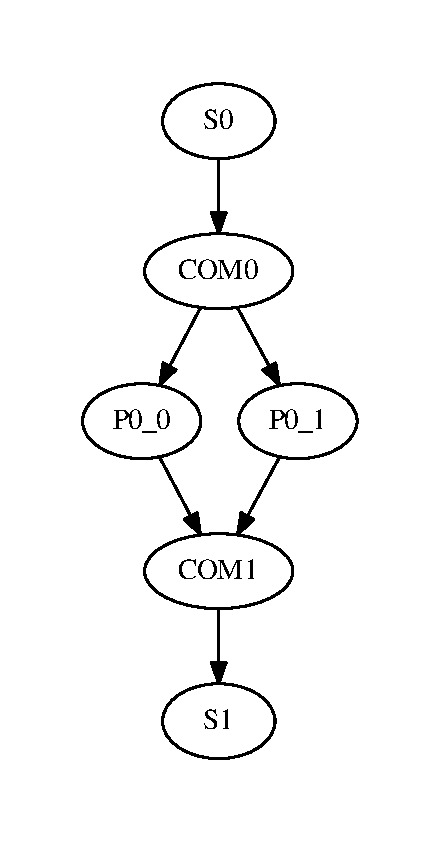
\includegraphics[scale=0.5]{figures/trans_cfg}
\caption{Transformed task graph based on mapping in Figure~\ref{f:distr_tg}. The serial portions are denoted by S, the parellel portions by P, and communication overhead by COM.}
\label{f:trans_cfg}
\end{figure}

Priority assignment will be done first on a task by task basis, and then on a function by function basis. The task priority assignment will first be done according to standard SMC practices by assigning the lowest priority to the task with the latest deadline. If a task is running on two cores then it must be the lowest priority on \emph{both cores} before being selected. There may of course still be both a low and high criticality candidate. With priorities assigned for each task, then parallel tasks must be further decomposed into several subtasks. The priority of each subtask must be assigned such that:
\begin{itemize}
 \item Any sub-task belonging to the same task that executes on the same core and that has precedence must have a higher priority.
 \item The set of tasks which have higher priority and lower priority must be the same for all subtasks as for the parent task (excluding the subtasks themselves).
 \item Each subtask has the same $L_i$ $T_i$ and $D_i$ as the parent task.
\end{itemize}

Let the set of all subtasks belonging to the same task $\tau_i$ be denoted $\bar{\tau_i}$. The response time $R_i$ is decomposed into serial and parallel sections. The response time for a serial section is simply:
\begin{equation}
R_{i(s)} = C_{i(s)} + \sum_{\tau_j \in hp(i)\backslash \bar{\tau_i} } \left\lceil\frac{R_{i(s)}}{T_j} \right\rceil C_j(L_i)
\end{equation}
Note that the set of higher priority tasks considered does not include sub-tasks belonging to the same priority. 
For parallel branches that begin at the same time, the maximum of all the branches must be taken:

\begin{equation}
R_{i(p)} = \max\limits_{k}\left\{ 
C_{i(pk)} + \sum_{\tau_m \in hp(i)\backslash \bar{\tau_i} } \left\lceil\frac{R_{i(pk)}}{T_m} \right\rceil C_m(L_i)
\right\}
\end{equation}

The response time is the sum of all the parallel and serial sections of the task:

\begin{equation}
R_i = \sum(R_{i(s)} + R_{i(p)})
\end{equation}

With this definition, only the parts of a divided task that are on the same core will have an impact on the response time. The effect of having two serial functions that belong to a higher priority task execute on a core is the same as having two independent tasks with the same period $T_i$ and combined execution time $C_i$.

With a schedulability analysis in place, it is possible to do DSE to find a legal mapping. \textbf{It remains to be determined whether this extra degree of freedom results in more schedulable systems at higher utilizations, and how this relationship is affected by the shape of individual CFGs, the amount of branching, and the communication overhead.} 

Typical multicore scheduling algorithms are categorized as either partitoned or global. Global scheduling assigns tasks to cores at runtime from a global queue. Partitioned algorithms statically allocate tasks to cores at design time while still allowing for the sporadic generation of new jobs by each task. This application model and scheduling algorithm is closer to partitioned scheduling. The resources consumed by a task are statically assigned however a task is no longer restricted to consuming a single resource. Tasks will consequently take advantage of coarse-grained parallelism in its dataflow to provide different performance or energy tradeoffs. Further tradeoffs may also be discovered when integrating reliability concerns into the mixed-criticality discussion.

\subsection{Mixed-criticality fault-tolerant schedulability analysis (MCFTS)}
The basic language for MC multicore schedulability can be used to extend mixed-criticality scheduling to include fault tolerance. First, we define the \textbf{task model}:
\begin{equation}
\tau_i=<T_i,L_i,C_i(L),D_i,pFH(L_i)>
\end{equation}
where:
\begin{itemize}
  	\item $T_i$: frequency of task
	\item $L_i$: criticality of task
	\item $C_i$: mode-dependent execution time of task
	\item $D_i$: deadline of task
	\item $pFH$: criticality-dependent maximum allowable probability of failure/hour
\end{itemize}

Second, we define the \textbf{processor model}:
\begin{equation}
\pi_i = <E_i,v_i,f_i,d_i,c_i,r_i,hw_i>
\end{equation}
where: 
\begin{itemize}
  \item $E_i$: energy profile
  \item $v_i$: operating frequency
  \item $f_i$: probability of transient fault
  \item $d_i$: availability of internal detection mechanism
  \item $c_i$: availability of internal correction mechanism
  \item $r_i$: recovery overhead
  \item $hw_i$: hardware profile (e.g. has FPU, has fingerprint unit, etc.)
\end{itemize}


\begin{table}
\centering
\caption{Example task set}
\begin{tabular}{@{}l|ccccc@{}} 
\toprule
		& C(LO) & C(HI) & T=D & L & P	 \\\bottomrule
$\tau_1$ & 5 & 10 & 25 & HI & 3 \\
$\tau_2$ & 5 & - & 20 & LO & 4 \\
$\tau_3$ & 2 & - & 8 & LO & 1 \\
$\tau_4$ & 1 & - & 5 & LO & 2 \\
\end{tabular}
\label{t:exampletask}
\end{table}


Consider the example task set provided in Table~\ref{t:exampletask}. We wish to determine whether it is possible to execute the task set on a two-core platform. The safety of the system will depend on the required level for each criticality level as well as the predicted rate of transient errors per core. We assume that some dependable runtime mechanism exists for keeping track of the actual number of transient faults per hours of operation. It is also assumed that each node is capable of detecting errors. In this case two values are defined: $f(LO)$ is the predicted rate of soft errors and $f(HI)$ is a more conservative estimate to be used in the case that a higher error rate than $f(LO)$ is detected in the field. It is possible that the ratio $\frac{f(HI)}{f(LO)}$ is provided by a safety standard.

Each HI level task also has two execution times $C(LO)$ and $C(HI)$. Four criticality modes naturally emerge from the fact that both $f$ and $C$ have two possible values. The four modes are:

		\begin{enumerate}
		  \item \textbf{$LO_cLO_f$}: Default mode. All tasks complete within maximum number of retries and within $C_i(LO)$.
		  \item \textbf{$LO_cHI_f$}: The predicted $f_i$ on processor $\pi_i$ is surpassed. More retries must be scheduled for HI tasks.
		  \item \textbf{$HI_cLO_f$}: The execution time of a task exceeds its $C_i(LO)$. In this case more time must be allotted for the execution of each task and its retries.
		  \item \textbf{$HI_cHI_f$}: Both the measure execution time and frequency of transient faults exceed their LO values.
		  \end{enumerate}
		  
Suppose that $f(LO)=10^{-5}$ and $f(HI)=10^{-3}$. Furthermore, suppose that $pFH(LO)$ is given to be $10^{-3}$ and $pFH(HI)=10^{-8}$. It should be immediately clear that there is a problem since $pFH(HI)>f(LO)$ as well as $f(HI)$. The solution to this problem is to re-execute the the HI level task $\tau_{1}$. If a task $\tau_i$ has utilization $u_i = \frac{C_i}{T_i}$ and is running on a processor with $f_i$ then $pFH_i=u_if_i$. Assuming that each run is independent, then executing a task n times results in an overall probability of failure:
\begin{equation} 
pFH_i(n)=(u_if_i)^n
\end{equation}
In this case, the minimum number of re-executions can be determined:
\begin{equation}
n \geq \frac{log(pFH_{L_i})}{log(u_if_i)}
\end{equation}
It is now possible to determine the minimum number of executions of $\tau_1$ for each mode:
\begin{equation}
   (U_1(LO)f_1(LO))^n=(0.2*10^{-5})^n \leq 10^{-8} \rightarrow n \geq 1.40
\end{equation}
\begin{equation}
   (U_1(HI)f_1(LO))^n=(0.4*10^{-5})^n \leq 10^{-8} \rightarrow n \geq 1.48
\end{equation}
\begin{equation}
   (U_1(LO)f_1(HI))^n=(0.2*10^{-3})^n \leq 10^{-8} \rightarrow n \geq 2.1
\end{equation}
\begin{equation}
   (U_1(HI)f_1(HI))^n=(0.4*10^{-3})^n \leq 10^{-8} \rightarrow n \geq 2.35
\end{equation}

	The result is that only one replica is needed so long as the $f(LO)$ threshold is not exceeded. Otherwise, two replicas are needed. The task set is updated in Tables \ref{t:exampletask2} and \ref{t:exampletask3}.

\begin{table}
\centering
\caption{Updated task set for modes $LO_cLO_f$ and $HI_cLO_f$}
\begin{tabular}{@{}l|ccccc@{}}
\toprule
		& C(LO) & C(HI) & T=D & L & P	 \\\bottomrule
$\tau_1$ & 5 & 10 & 25 & HI & 3 \\
$\tau_1'$ & 5 & 10 & 25 & HI & 4 \\
$\tau_2$ & 5 & - & 20 & LO & 5 \\
$\tau_3$ & 2 & - & 8 & LO & 1 \\
$\tau_4$ & 1 & - & 5 & LO & 2 \\
\end{tabular}
\label{t:exampletask2}
\end{table}

   \begin{table}
\centering
\caption{Updated task set for modes $LO_cHI_f$ and $HI_cHI_f$}
\begin{tabular}{@{}l|ccccc@{}}
\toprule
		& C(LO) & C(HI) & T=D & L & P	 \\\bottomrule
$\tau_1$ & 5 & 10 & 25 & HI & 3 \\
$\tau_1'$ & 5 & 10 & 25 & HI & 4 \\
$\tau_1''$ & 5 & 10 & 25 & HI & 5 \\
$\tau_2$ & 5 & - & 20 & LO & 6 \\
$\tau_3$ & 2 & - & 8 & LO & 1 \\
$\tau_4$ & 1 & - & 5 & LO & 2 \\
\end{tabular}
\label{t:exampletask3}  
\end{table}
   
Once the task sets have been updated, standard schedulability analysis can be carried out with AMC-rtb and partitioned core allocation. The replicas are modelled as a parallel set stemming from a source and sink with zero cost.

\subsection{MCFTS and on-demand redundancy}

The processor model allows for the existence of internal detection or correction mechanisms. These mechanisms may be expensive and difficult to scale and may not be available on every core in a system. On-demand redundancy (ODR) \cite{c} suggests it is possible to run replicas on two unprotected cores in order to detect an error by comparing their outputs. The cores may otherwise execute independently when working on non-critical tasks. There are proposed mechanisms \cite{c} to allow the dynamic pairing of cores over long distances as well as studies examining the benefits to overall performance in a non-embedded setting \cite{c}. 
   
   \begin{figure}
\centering
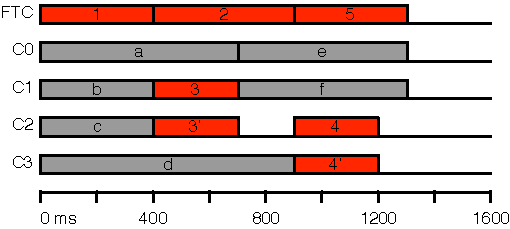
\includegraphics[scale=1]{figures/schedule-dcc.pdf}
\caption{System scheduling using ODR and DCC. Non critical tasks are depicted in grey and critical tasks are depicted in red.}
\label{f:schedule-dcc}
\end{figure}


   On demand redundancy is illustrated in Figure~\ref{f:schedule-dcc}. The system contains one fault-tolerant core (FTC) which is assumed to have dependable internal detection or correction mechanisms. The other cores are assumed to be some combination of smaller, more powerful, and more energy efficient because they are unburdened with extra fault-tolerance logic. Cores C1 and C2 execute non-critical tasks independently. They are then coupled to execute Task 3 and its replica in parallel. This is equivalent to a single replica with error detection assumed to take place within the node in the previous section.
   
   The probability of a task failing is slightly different now that it depends on the execution of two nodes, each with their own $f_i$. A task $\tau_i$ executing on two cores $\pi_j$ and $\pi_k$ will have a new failure rate:
   \begin{equation}
   f_{jk} = 1 - (1-u_if_j)(1-u_if_k)
   \end{equation} 
That is 1 minus the probability that neither processor has a transient fault (assuming faults on each core are independent).
   
   
%%%%%%%%%%%%%%%%%%%%%%%%%%%%%%%%%%%%%%%%%%%%%%%%%%%%%%%%%%%%%%%%%%%%%%%%%%%%%%%%%%%%%%%%%%%%%%%%%%%%%%%%%%%%%%%%


\section{Code Profiling}
\subsection{Parsing}
The profiling tool determines maximum stack size required by a function as well as its WCET to map the application to hardware resources and prove schedulability. The tool takes as input the disassembly file generated by \texttt{nios2-elf-objdump} as well as the root function to be analyzed. Listing \ref{l:prof_input} demonstrates how to correctly generate the disassembly and run the profiler. The user should eventually be able to run a series of profiles on various functions using a configuration file. 


\begin{lstlisting}[caption={Generating disassembly and running the profiler},label=l:prof_input]
$ nios2-elf-objdump -dt filename.elf > filename.objdump
$ java Profiler filename.objdump top_level_function
\end{lstlisting}

The parser works in several passes. First, function names are extracted from the \texttt{objdump} file. The next few passes build the control flow graph (CFG). The code associated for each function is broken down into basic blocks. Calls, returns, branches, and jumps are identified as the end of basic blocks. The parser can now identify which functions are called by other functions. All functions that are not called from the root are removed from the analysis at this point. Following this pruning of the CFG, the basic blocks are further divided because branch, jump and call \emph{destinations} must be the start of basic blocks. Finally loops are identified by calculating the \emph{maximum depth} of each basic block. A backwards edge occurs in the case that a successor has a lower depth. The parser finally ouputs a \texttt{dot} file that can be compiled into a \texttt{pdf}. Figure \ref{f:parse_flow} depicts the parser workflow. Figure \ref{f:exdot} contains an example of the \texttt{dot} file.
 
\begin{figure} 
\centering
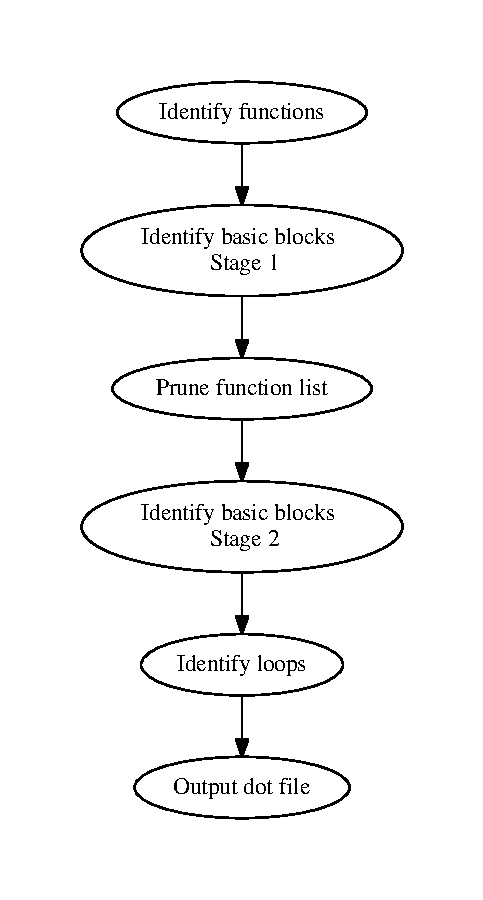
\includegraphics[scale=0.6]{figures/parse_flow.pdf}
\caption{Parser workflow}
\label{f:parse_flow}
\end{figure}

\begin{figure}  
\centering
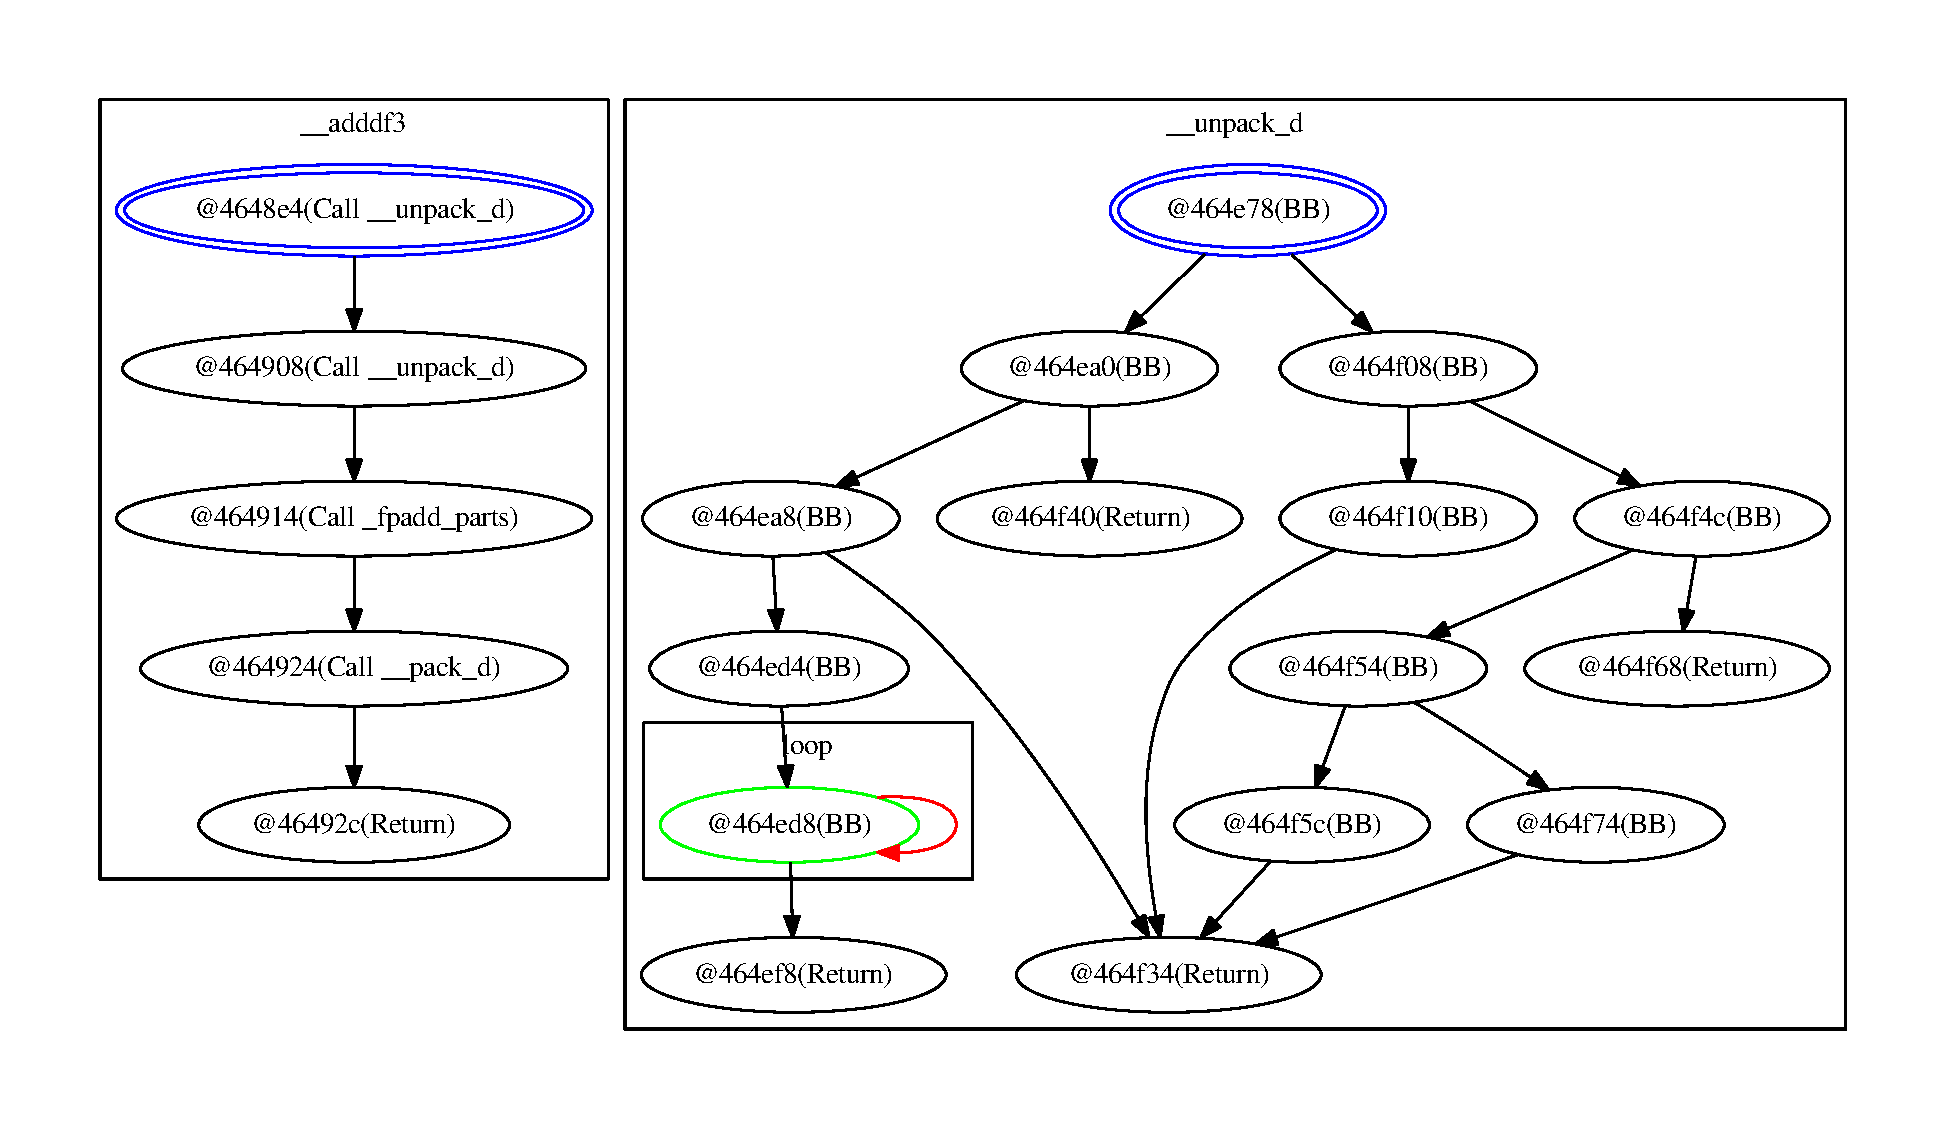
\includegraphics[scale=0.4]{figures/cfg.pdf}
\caption{Example of visual CFG representation generated by the parser}
\label{f:exdot}
\end{figure}



\subsection{Stack Analysis}
It is possible to start analysis once the parser has built the CFG. Stack analysis is quite straightforward. Each basic block in a function is checked for instructions that increase the stack size. Note that stack instructions should not occur in a loop. If a basic block calls a function, then that function is also checked for stack instructions and then this result is added on to the original calculation. Recursive functions are not supported.

\subsection{Library functions}
Library functions are important because they must be copied into the scratchpad along with the rest of the critical code. The library as well as the object that contains the function must be known in order to efficiently modify the linker script. All the library functions can be placed in a contiguous portion of memory for easy DMA transfer. The library directory for the default compiler used by the Nios II Software Build Tools (SBT) is located at: 

\texttt{altera/13.1/nios2eds/bin/gnu/H-i686-pc-linux-gnu/nios2-elf/lib}. 

These libraries have been copied to \texttt{code\_gen/nioslib} for convenience. The script \texttt{extract.sh} has been provided to extract object names and function names from each library. The main commands are explained in Listing \ref{l:extract}. Static objects mapping functions to their containing object files and library are then created in Java, as demonstrated in Listing \ref{l:jlib}.

\begin{lstlisting}[caption={Extracting information from shared libraries},label=l:extract]

# list the object files in an archive
ar -t $archive

# extract the object files from the archive
ar -x library.a

#create an objdump for each file.o 
nios2-elf-objdump -d file.o > file.objdump

#Extract the function names for each object file
grep "<.*>:" $f.objdump | sed -r 's/.*<(.*)>:/\1/' >> $OUTPUT

\end{lstlisting}

\begin{lstlisting}[caption={Extracting information from shared libraries},label=l:jlib,language=Java]
 
static HashMap<String, String> libc = new HashMap<>();
	static {
		libc.put("memset", "lib_a-memset.o");
		libc.put("critical_factorization", "lib_a-memmem.o");
		etc...
	}

\end{lstlisting}

The output from the library analysis is a code listing that can be added inside a region in the linker script to place those functions. 

\begin{lstlisting}[caption={Placing library functions in \texttt{.critical} region},label=l:jlib,language=C]
/* Library functions are: __muldf3,__muldi3,__pack_d,__unpack_d,__mulsi3,__lshrdi3,__ashldi3 */
/* To place these functions in a section called critical in linker.x: */
    .critical :
    {
        PROVIDE (_alt_partition_critical_start = ABSOLUTE(.));
        *(.critical .critical.*)
        
        /* INSERT THE FOLLOWING */
        
        */libgcc:_mul_df.o
        */libgcc:_unpack_df.o
        */libgcc:_pack_df.o
        */libgcc:_lshrdi3.o
        */libgcc:_ashldi3.o
        */libgcc:_muldi3.o
        */libgcc:lib2-mul.o
        
        /* END OF INSERTED CODED */
        
        . = ALIGN(4);
        
        PROVIDE (_alt_partition_critical_end = ABSOLUTE(.));
    } > processor0_0_scratchpad


\end{lstlisting}


\subsection{Worst case execution time estimation}
The WCET for a function is calculated using implicit path enumeration technique (IPET) \cite{Li:1995:PAE:216636.216666}. IPET is a method of pessimistically determining the WCET of a
program without actually identifying the worst-case path. The first step is to convert the CFG into an integer linear program (ILP) and the second step is to determine the cost of each basic block using microarchitectural modelling and/or dataflow analysis. 

The goal of the ILP is to maximize the objective function:

\begin{equation}
\sum_{i=1}^{N}c_ix_i
\end{equation}

where:

\begin{itemize}
  \item $N$: Number of basic blocks
  \item $c_i$: Execution time of block $i$
  \item $x_i$: frequency of block $i$
\end{itemize}

The CFG is transformed into a set of linear constraints by noting that the number of times a basic block is entered must equal the number of times it is exited. Each edge in the CFG is assigned a variable $e_i$. The entry edge into the root basic block has the constraint $e_0 = 1$. For all other edges, constraints are extracted based on the observation that for each basic block: $\sum e_{in} - \sum e_{out} = 0$. For example, in Figure~\ref{f:bbedges}: $e_0+e_1+e_2-e_3=0$.

\begin{figure}[h]
\centering
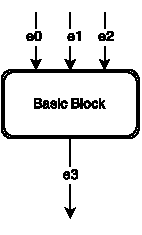
\includegraphics[scale=1]{figures/bbedges.pdf}
\caption{Sum of the edges into the basic block must equal the sum of the edges out: $\sum e_{in} - \sum e_{out} = 0$.} 
\label{f:bbedges}
\end{figure}


% Loops require an additional constraint on the maximum number of times the loop can can run. Therefore for each loop $\sum e_{in} \leq m$ where $m$ is the maximum number of iterations. In Figure~\ref{f:loopedges}, taking $m=10$ gives: $e_0 + e_1 + e_2 + e_4 \leq 10$. Functions calls are not explicitly represented in the constraint system. Each function is analyzed independently and then the final execution time of a basic block $i$ that calls function $f$ is defined as: 
%   $(c_i+WCET(f))x_i$. Recursive function calls are not supported but are also generally not used in real-time systems.


Loops require an additional constraint on the maximum number of iterations. Therefore for each loop $\sum e_{in} - \sum \mathrm{maxIter}*e_{fl} \le 0$, where $\mathrm{maxIter}$ is the maximum number of iterations for the loop and $e_{fl}$ are the non-backwards edges into the loop (i.e. those that can only execute once per single round of loop iterations).


\begin{figure}[h]
\centering
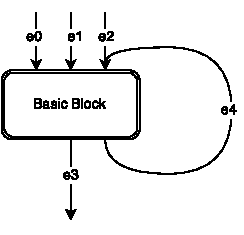
\includegraphics[scale=1]{figures/loopedges.pdf}
\caption{An additional constraint is required for loops: $\sum e_{in} \leq m$.} 
\label{f:loopedges}
\end{figure}


Function calls are handled quite simply. The entry-point to the top-level function simply equals 1. For all other functions, the entry-point equals the sum of all the edges leaving basic blocks that call that function. In Figure~\ref{f:function-ipet}, the result is: $e_2+e_3-e_4 = 0$.

\begin{figure}[h]
\centering
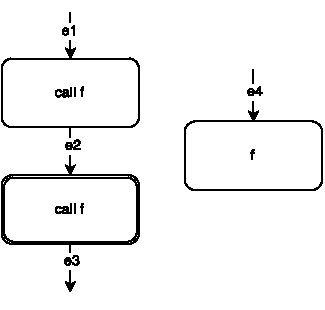
\includegraphics[scale=1]{figures/function-ipet.pdf}
\caption{The sum edges leaving function call blocks is equal to the edge entering that function's root block.} 
\label{f:function-ipet}
\end{figure}
 


Library functions are difficult to analyze. Loops can be identified but their bounds cannot be easily determined analytically without detailed dataflow analysis beyond the current scope of the tool. An attempt was made to analyze the WCET of floating point operations by observing the number of times a loop executed in an OVP simulation environment. This information is then be used with associated microarchitectural modelling to come up with a cycle accurate estimation. There is no way to prove that the maximum observed loop iterations (over thousands of randomized trials) is in fact an upper boundary. Furthermore, it is a known problem that IPET yields pessimistic results if some paths through the control flow are impossible (but this is difficult to detect without detailed dataflow analysis). 


\begin{figure}[h]
\centering
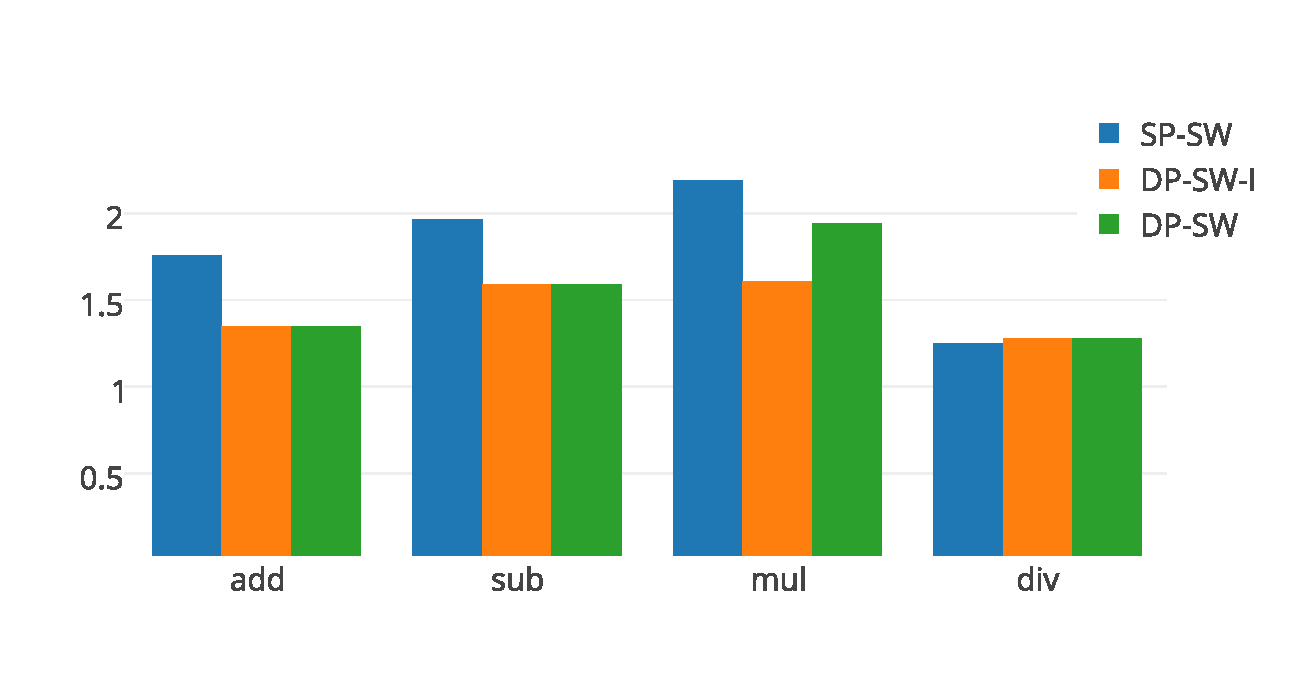
\includegraphics[scale=0.5]{figures/ipetresults}
\caption{The results from IPET analysis compared to worst-case measured in OVP simulation.}
\label{f:ipetresults}
\end{figure}


Figure~\ref{f:ipetresults} shows the WCET calculated using IPET normalized to the measured execution time (maximum number of instructions observed in OVP) for all four operations. The OVP simulation provided boundaries for the library function loops. Single-precision is tested without integer multiplication hardware (SP-SW). Double precision is tested with integer multiplication hardware (DP-SW-I) and without (DP-SW). This chart demonstrates that software-based floating point operations are a source of imprecision that is difficult to overcome. 
For regular control flow, IPET will only be as effective as the hints provided by the programmer.

This result has motivated the inclusion of FPUs in the processing cores. The FPU provided by Altera executes single precision operations using the custom instruction interface to the Nios II. Each instruction has a known execution time in clock cycles which eliminates the pessimism in calculating floating point operations. It is possible to force Simulink to generate code using only single precision variables and operations. As a result, there is a tradeoff between the accuracy of the WCET estimation, the size of the core (inclusion of an FPU), and limiting calculations to single-precision. The FPU will also remove thousands of instructions from the critical function and reduce the interference due to instruction loads from main memory as well as lower execution time considerably.

\subsection{Microarchitectural modelling}

 
%%%%%%%%%%%%%%%%%%%%%%%%%%%%%%%%%%%%%%%%%%%%%%%%%%%%%%%%%%%%%%%%%%%%%%%%%%%%%%%%%%%%%%%%%%%%%%%%%%%%%%%%%%%%%%%%
\section{Application Mapping}

The initial scheduling algorithm will be taken from Bolchini and  Miele \cite{bolchini2013reliability}. A genetic algorithm (GA) is used to explore the design space. The general details that follow on genetic algorithms are based on the overview in \cite{geatbx}.

Figure \ref{f:ga_ov} shows an overview of how to implement a genetic algorithm. There are two stages of GA in the given process. First tasks must be organized into groups of tasks, and each group of tasks must be assigned a fault detection technique or fault tolerance technique. DMR Fingerprinting is an example of a detection mechanism. This work will remain agnostic about the method of implementation of fault tolerance. We assume that appropriate hardening measures are applied to a single core.
 
\begin{figure}[h]
\centering
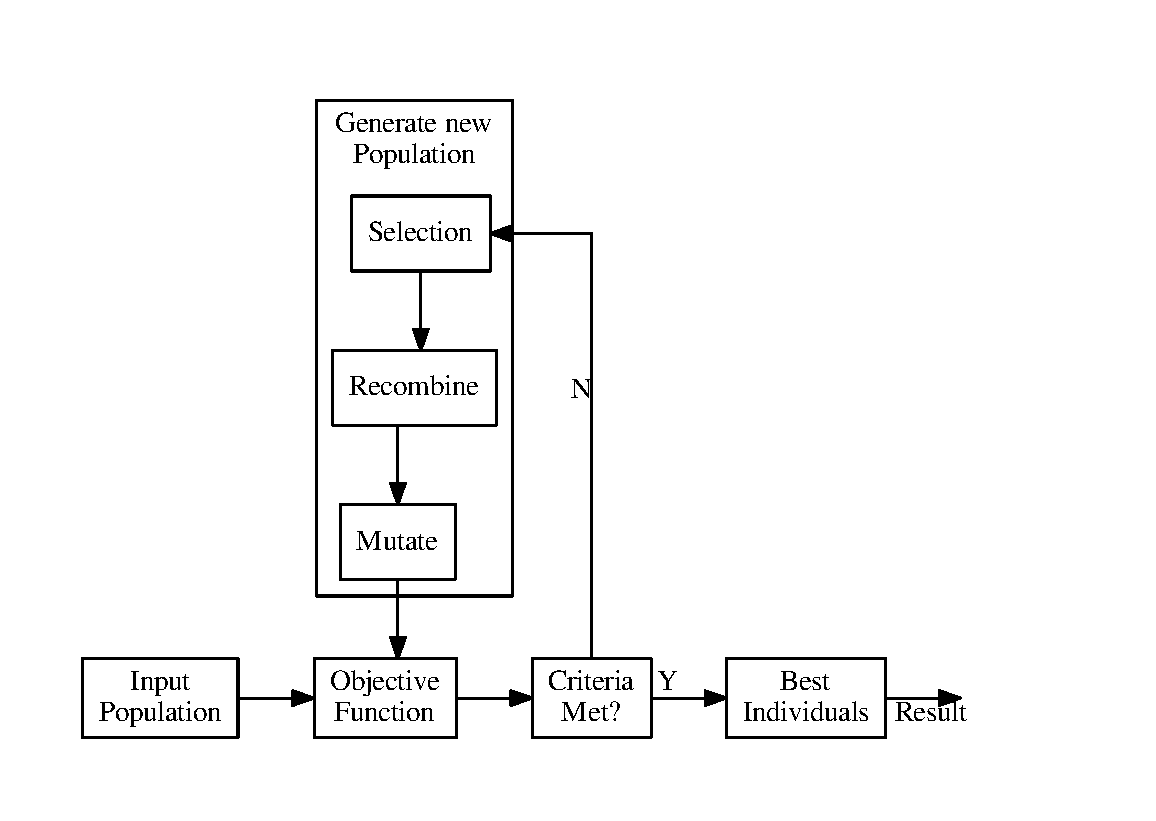
\includegraphics[width=12cm]{figures/ga_ov}
\caption{The basic structure of a genetic algorithm \cite{geatbx}.}
\label{f:ga_ov}
\end{figure}

Once a population of various groupings and associated fault-handling mechanisms has been generated it is necessary to test their fitness. This must be done by generating a system schedule for each member of the population. 

The generation of the schedule is itself done with a second round of GA. Each task is assigned to an appropriate core based on the fault-handling requirements of its group. The group adopts the most stringent requirements of any of its members. Various mappings are generated as the GA population. Then it is necessary to order the tasks on each core. This is complicated by the fact that there may be inter-core data dependencies. For now, we will neglect the overhead associated with data transfer between cores.

The first step for scheduling on each core once groups have been assigned is to generate a list of tasks for which all the start conditions have been met (i.e. data dependencies on previously executed tasks). The highest priority task is chosen from this list for each core. This process cycles through all the cores and then proceeds to the next event in time (i.e. a task has ended) to repeat the process. 

The priority of a task is determined using \emph{modified partial critical path priority} \cite{eles2000scheduling}. The method consists of choosing tasks that minimize the critical path on \emph{other cores}. It is possible that a successor to a task will be in the pool of tasks. Therefore, the critical path length is only considered from the first successor task that will execute on a different core. 

Consider the example from \cite{eles2000scheduling} in Figure~\ref{f:crit_path}. From a start point $P_0$, either task $P_A$ or $P_B$ must be selected. The chain of tasks from $P_A$ to $P_X$ represents a series of successor tasks that will all be executed on the same core in time $t_A$. The time $\lambda_A$ represents the time from the first successor on a different core to the terminal or sink task $P_N$. The scheduler must determine whether to assign $P_A$ or $P_B$ higher priority. This is done by choosing the option that minimizes the critical path \emph{on other cores}. This means that $t_A$ and $t_B$ are neglected and the path with shorter $\lambda$ is chosen. One interesting question is whether it would be simpler and more effective on a system with \emph{many} cores to simply choose the task with the largest number of critical children nodes or non-critical children nodes (in that order) since this will most likely facilitate parallel execution on a large system.

\begin{figure}[h]
\centering
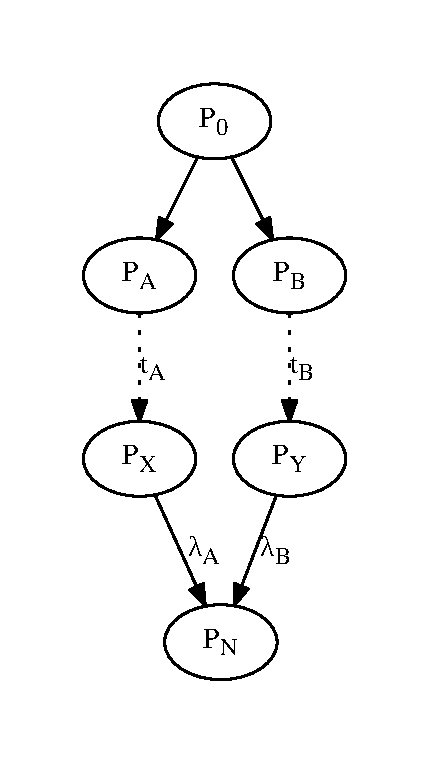
\includegraphics[scale=0.7]{figures/crit_path}
\caption{Example of modified partial critical path priority selection \cite{eles2000scheduling}.}
\label{f:crit_path}
\end{figure}



The implementation details of the genetic algorithm will be adopted from \cite{bolchini2013reliability}. Tournament selection and single-point crossover operator recombination will be used. Mutations will be applied randomly. There are four mutations at the task level: change the group of a task, split a group in two, join two groups, or change the fault-management technique applied to a group. The mutation for the mapping phase consists of switching a task to another processor that can meet the assigned fault-management requirements.

Tournament selection means choosing a subset of the population and selecting the most fit member. This is repeated as many times as necessary. Single-point crossover cuts two parent chromosomes into two pieces and then exchanges the second substrings between the chromosomes. 

The initial parameters for the GA will be the ones suggested in \cite{bolchini2010multi}. The crossover rate is 80\%, the mutation rate is 10\%. The program will run for 30 generations. The population size will be between one and two thousand.

The JGAP library \cite{jgap} is used to implement the genetic algorithm. 

\subsection{Recovery}
Fault model: can't fail twice.
Need to leave room for reexecution. 
Fill up the retry slots with soft tasks. Just cancel them if the retry slot is needed.

Recovery only necessary in the case of correction. Detection implies no retry. 

Why? Application where delivering the wrong answer can be catastrophic but dropping a frame is acceptable (i.e. not sensitive to jitter)



%%%%%%%%%%%%%%%%%%%%%%%%%%%%%%%%%%%%%%%%%%%%%%%%%%%%%%%%%%%%%%%%%%%%%%%%%%%%%%%%%%%%%%%%%%%%%%%%%%%%%%%%%%%%%%%%
\section{Code Generation}

\subsection{Code templates}

This tool is designed to convert code generated by Matlab into a working and estimate safe properties for a mutlicore Nios system. The baseline architecture is depicted in Figure~\ref{f:nios-arch}. 

\begin{figure}[h]
\centering
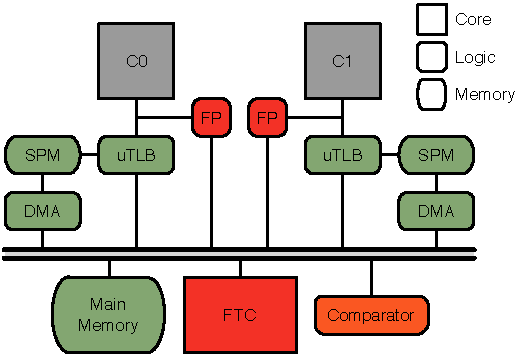
\includegraphics{figures/architecture.pdf}
\caption{The baseline architecture for the generation tool}
\label{f:nios-arch}
\end{figure}

A fault-tolerant core (FTC) (assumed to have internal detection and/or correction mechanisms to manage soft errors) monitors execution on less reliable cores. Code must be generated for message passing, thread migration, bus management, memory management, runtime monitoring and reliability management. A breakdown of the generation templates will follow using the example Simulink generated control system, prepared as part of an undergraduate design project, in Figure~\ref{f:simulink}.

\begin{figure}[h]
\centering
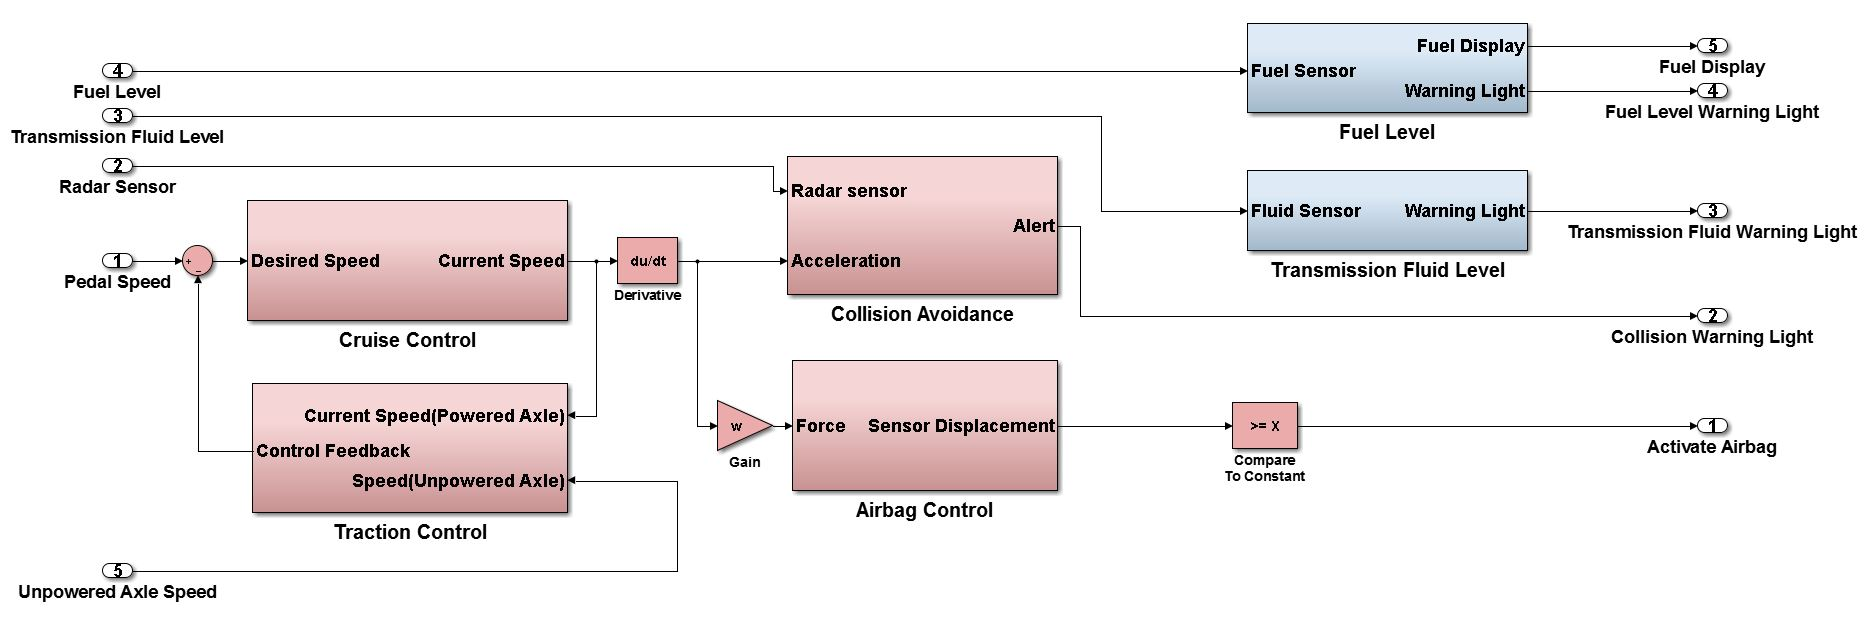
\includegraphics[scale=0.32]{figures/matlab-ctrl.jpg}
\caption{Example control system from Simulink}
\label{f:simulink}
\end{figure}

The control sytem is broken up into seven tasks:

\begin{itemize}
  \item Cruise control and adder
  \item Traction control
  \item Derivative
  \item Gain, airbag control and compare
  \item Collision avoidance display
  \item Transmission fluid level display
  \item Fuel level display
\end{itemize}

The three display related functions are considered non-critical. The other functions are critical as they relate to airbag activation. For this example all critical tasks must execute every 20ms, while non-critical tasks execute every 100ms.

\subsubsection{Monitor tasks}
The monitor tasks must run on the FTC. They consist of:
\begin{itemize}
  \item setting up task parameters and initializing all critical task models
  \item managing dataflow between tasks 
  \item intercore task communication 
  \item retrieving valid data when critical tasks execute correctly on other resources 
  \item restarting cores in the case of a transient fault
  \item managing the global data space
  \item organizing coordinated virtual memory management and memory protection between cores to achieve correct fingerprinting
\end{itemize} 

Figure~\ref{f:monitor-send} shows a high-level view of how the interaction between monitor tasks in order to send a message.

\begin{figure}
\centering
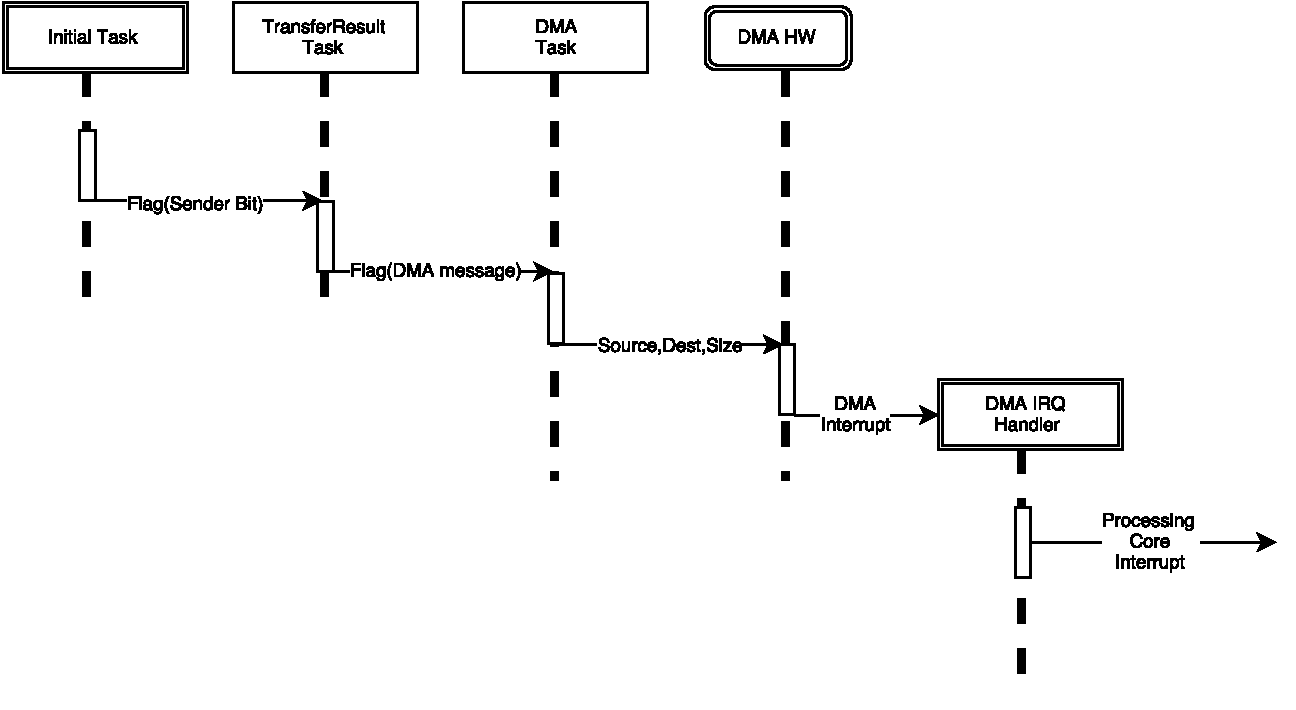
\includegraphics[scale=0.7]{figures/monitor-send.pdf}
\caption{The interaction between monitor tasks when setting up a critical task to run on another core}
\label{f:monitor-send}
\end{figure}

\textbf{MODULARITY VS. CONTEXT SWITCH OVERHEAD $\rightarrow$ FUNCTIONAL VS. TASK-BASED DIVISION OF LABOUR???}

The monitor is responsible for ensuring that 

\subsubsection{Integration of Simulink generated code}

The code generated from the Simulink model will dictate how to structure the communication between tasks. Functions must be generated using the reusable code option and using the input and output structures option. Discrete models must be used for Nios compatibility.

\todojc{show simulink options menu figure here}
There are three functions generated for each group of blocks: an initalization, a termination, and a step function. Example function declarations are shown in Listing~\ref{l:airbag-proto} along with the struct definitions for the input parameters. There are three different parameters for all the function: 
\texttt{RT\_MODEL\_AirbagModel\_T} stores the state that is needed between time steps, \texttt{ExtU\_AirbagModel\_T} stores the external input parameters, and \texttt{ExtY\_AirbagModel\_T} stores the external outputs. The members of each input and output struct must either connect to inputs and outputs of other functions or communicate somehow with on-chip peripherals or through IO. The connection to IO is not currently implemented.

\begin{lstlisting}[caption={Airbag model function declarations},label=l:airbag-proto,language=C]
/* Model entry point functions */
extern void AirbagModel_initialize(RT_MODEL_AirbagModel_T *const AirbagModel_M,
  ExtU_AirbagModel_T *AirbagModel_U, ExtY_AirbagModel_T *AirbagModel_Y);
extern void AirbagModel_step(RT_MODEL_AirbagModel_T *const AirbagModel_M,
  ExtU_AirbagModel_T *AirbagModel_U, ExtY_AirbagModel_T *AirbagModel_Y);
extern void AirbagModel_terminate(RT_MODEL_AirbagModel_T *const AirbagModel_M);
\end{lstlisting}

In Figure~\ref{f:simulink} the cruise control outputs a single \texttt{real\_T} value (Listing~\ref{l:cc-output}) and the derivative function has an identical input (Listing~\ref{l:der-input}). The monitor will need to pass the signals between the data structures.
\begin{lstlisting}[caption={Cruise control output struct definition},label=l:cc-output,language=C]
/* External outputs (root outports fed by signals with auto storage) */
typedef struct {
  real_T Out1;                         /* '<Root>/Out1' */
} ExtY_CruiseControlSystem_T;
\end{lstlisting}

\begin{lstlisting}[caption={Derivative input struct definition},label=l:der-input,language=C]
/* External inputs (root inport signals with auto storage) */
typedef struct {
  real_T In1;                          /* '<Root>/In1' */
} ExtU_Derivative_T;
\end{lstlisting}

There will be two more levels of packaging for the monitor that will be used later on for convenient DMA transfers. First, all three structs will be packaged in a single container. Then, for all critical tasks that will require DMA transfer and that have precedence relations between them (i.e. the completion of one triggers the beginning of the next), they will be placed in a single struct so that the DMA can transfer data with a single command. The structs, presented in Listing~\ref{l:dma-struct}, are not all located in the same file. The model contains pointers that must be assigned to static variables manually. Examples are located in the \texttt{ert\_main.c} file accompanying each generated project.

\begin{lstlisting}[caption={Structures of structures to facilitate DMA transfer.},label=l:dma-struct,language=C]
/* LOCATED IN critical.h */
typedef struct {
	RT_MODEL_Derivative_T Derivative_M;
	ExtU_Derivative_T Derivative_U;
	ExtY_Derivative_T Derivative_Y;
} DerivativeStruct;

typedef struct {
	RT_MODEL_AirbagModel_T AirbagModel_M;
	ExtU_AirbagModel_T AirbagModel_U;
	ExtY_AirbagModel_T AirbagModel_Y;
} AirbagModelStruct;

/* LOCATED in monitor main.c */
typedef struct {
	AirbagModelStruct airbagModelStruct_0;
	DerivativeStruct derivativeStruct_0;
} DMAPackageStruct;
\end{lstlisting}






%%%%%%%%%%%%%%%%%%%%%%%%%%%%%%%%%%%%%%%%%%%%%%%%%%%%%%%%%%%%%%%%%%%%%%%%%%%%%%%%%%%%%%%%%%%%%%%%%%%%%%%%%%%%%%%%

\section{References}

\begingroup
\renewcommand{\section}[2]{}%
\bibliographystyle{ieeetr}
\bibliography{codegen}
\endgroup

\end{document}